\documentclass[11pt]{article}

% Packages
\usepackage[utf8]{inputenc}
\usepackage[margin=1in]{geometry}
\usepackage{graphicx}
\usepackage{amsmath}
\usepackage{amssymb}
\usepackage{booktabs}
\usepackage{hyperref}
% \usepackage{natbib}  % Uncomment if using .bib file with bibtex
\usepackage{float}
\usepackage{caption}
\usepackage{subcaption}
\usepackage{tikz}
\usetikzlibrary{shapes.geometric, arrows.meta, positioning, fit, backgrounds}

% Single spacing
\usepackage{setspace}
\singlespacing

% Title information
\title{Marvel Rivals Win Prediction and Hero Recommendation}
\author{
    Robert Moore \\
    \texttt{robert.moore.593@my.csun.edu}
    \and
    Ken Douglas \\
    \texttt{kenneth.douglas.994@my.csun.edu}
    \and
    Behrouz Barati B \\
    \texttt{b3h@me.com}
}
\date{December 12, 2025}

\begin{document}

\maketitle
% ============================================================================
\section{Introduction}
Marvel Rivals is a third-person hero shooter where players battle in teams of 6 to accomplish various objectives, such as capturing checkpoints or safely escorting a moving object. As they face the enemy team and achieve or fail their objectives, each player accumulates statistics including damage dealt, KO's, Deaths, and more, which are gathered by integrated trackers and transmitted to online leaderboards along with the final match result. These statistics are the only objective record of a match, but their relationship to the final outcome is indirect and often unclear, making it difficult for, eg, an Esports coach to assess a prospective player's skill on the basis of their match history. Being able to make decisions off of simple statistics from a game is huge for the industry and a growing need in a data driven society. We sought to develop models that could accurately determine the outcome of a match based on these statistics. 

% ============================================================================

% Describe the problem
\subsection{Problem Description}
  
This project addresses the problem of predicting outcomes in competitive esports matches, where results depend on team composition, player impact, and in-game efficiency rather than a single statistic. To study this, a large collection of Marvel Rivals match logs was cleaned and standardized, resolving inconsistencies such as mixed time formats, zero-minute players, variable team sizes, and mid-match hero swaps.

After cleaning, match outcome prediction was formulated as a binary classification task. Engineered features capture team-level performance, role balance, and player impact, allowing a neural network to learn nonlinear relationships that answer key questions such as which team is likely to win and how composition and individual contribution influence match results.

% Describe the data
\subsection{Data Description}
We obtained a collection of match data by crawling the website rivalsmeta.com, which collates statistics from official trackers integrated into the game's various platforms (PC, PlayStation, and Xbox). Our crawler is written in Python, with the Playwright library being used to navigate the site and interact with dynamic page elements, while the BeautifulSoup library was used to parse the HTML into an easily-navigable DOM tree from which we could extract the relevant data. The crawler followed a breadth-first approach to locate new pages to scrape–it began with a few hand-selected public profiles of players near the top of the leaderboards, from which it pulled the data for every match they had played during the target time period. The data for each of these matches includes the identifiers of the player's teammates and opponents, all of which were added to a queue to be processed in the same manner as the original profiles. The process was repeated, while tracking which players' profiles had already been visited, eventually yielding data on 330,914 matches, including 458,565 unique players. Each match contains two teams, with player-level statistics such as damage, healing, deaths, hero usage, and rank. Players may swap heroes mid-match, resulting in variable hero counts per player. The target variable is a binary label indicating whether Team One or Team Two won the match. 

% Data preparation
\subsection{Data Preparation}
The first stage of my contribution was building a cleaning pipeline capable of preparing 330,914 matches for modeling. The major steps included:
\begin{itemize}
	\item 	Time normalization: Converting formats like “8.5m” or “45s” into consistent numeric minutes.
	\item 	Filtering invalid players: Removing players with 0 minutes played, since they introduce noise into per-minute calculations.
	\item	Enforcing team size: Some matches listed more than 6 players on a team; I kept only the 6 highest-minute players.
	\item 	Role mapping: Every hero was mapped into Tank, DPS, or Support, allowing role-share features.
\item Randomized flipping: With 50\% probability, I flipped the entire match (team\_one \(\leftrightarrow\) team\_two, scores, and winner).
This prevents the model from learning position-based shortcuts.
	\item 	Leakage prevention: Final score and round count were explicitly excluded from model input. 
\end{itemize}

By the end, the cleaned dataset captured a realistic competitive match environment with consistent structures across all matches. 

% Example figure placeholder
% \begin{figure}[H]
%     \centering
%     \includegraphics[width=0.8\textwidth]{figures/data_visualization.png}
%     \caption{Description of the visualization}
%     \label{fig:data_viz}
% \end{figure}

% ============================================================================
\section{Related Work}
% ============================================================================

\paragraph{Ken Douglas:}
Prior work has shown that match outcomes can be predicted accurately using engineered player- and team-level features rather than raw game logs, reinforcing the importance of feature engineering before model training~\cite{ref1}. The effectiveness of neural models combined with normalized performance metrics motivated my use of per-minute statistics, carry-style aggregates, and a sigmoid-based neural network output for win probability prediction.

Other studies have demonstrated that team composition alone, independent of in-game events, has a measurable impact on win probability~\cite{ref6}. While those approaches rely on search-based optimization, I adapt the core idea by using a trained neural network to dynamically evaluate and rank candidate hero picks during the draft phase.
\paragraph{Robert Moore}
I developed the web crawler independently based on my own research into what Python libraries would be most suitable for the task; in surveying the literature, I later found that the use of BeautifulSoup to parse HTML is fairly common \cite{scraping1} \cite{scraping2}, but I could not find any other instances of using Playwright for browser automation. The idea of developing player-specific models was inspired by PandaSkill \cite{pandaskill}, a framework used to rate players in the similarly team-based game League of Legends on the basis of individual performance. 

\paragraph{Behrouz Barati}
Gradient boosting and ensemble tree methods have demonstrated strong performance in esports match outcome prediction. Xiao et al.~\cite{xiao2021wpgbdt} proposed WP-GBDT, achieving 89.97\% AUC using gradient boosting decision trees with feature engineering on video game logs at IEEE BigData 2021. Akhmedov and Phan~\cite{akhmedov2021dota2} applied machine learning to Dota 2 match prediction, comparing Linear Regression (82\%), Neural Networks (88\%), and LSTM (93\%) using real-time game state data. Gourdeau and Archambault~\cite{gourdeau2020hero} developed discriminative neural networks for hero selection in MOBA games, demonstrating that team composition significantly impacts match outcomes. Our work extends these approaches by applying Random Forest, XGBoost, and CatBoost to Marvel Rivals and introduces a Retrieval-Augmented Generation (RAG) pipeline for natural language exploration of match statistics.

% ============================================================================
\section{Methods}
% ============================================================================

\subsection{Method 1: Neural Network (KD)}

\paragraph{Cleaning Pipeline.}
Over 310{,}000 Marvel Rivals matches were prepared through a custom cleaning pipeline.
Raw JSON logs were inconsistent and required preprocessing before modeling.
Key steps included time normalization, removal of zero-minute players,
enforcing six-player team limits, hero-to-role mapping (Tank/DPS/Support),
randomized team flipping with 50\% probability to remove positional bias,
and explicit exclusion of score-related fields to prevent target leakage.
The resulting dataset provides a consistent competitive structure across matches.

\paragraph{Feature Engineering.}
Team strength and player impact were represented using aggregated and normalized
features, including raw totals (damage, healing, deaths, kills, assists, final hits),
per-minute efficiency metrics (DPM, HPM, taken per minute),
role composition shares, hero swap and consistency measures, and known team-up synergies.
A deaths-aware carry score,
$\frac{\text{damage} + \text{taken} + \text{healed} + \text{final hits}}{\text{deaths} + 1}$,
was used to identify high-impact players regardless of role.
Statistical summaries (mean, max, standard deviation) were computed across players
to capture performance distribution within each team.

\paragraph{Neural Network Model.}
The predictive model is a two-hidden-layer neural network implemented in NumPy,
with approximately 94 input features, two hidden layers of 16 neurons each using
Leaky ReLU activations, and a sigmoid output producing Team One win probability.
This architecture balances expressive power with training efficiency and was chosen
to model nonlinear interactions such as role balance, hero synergy, and carry concentration.
Training used binary cross-entropy loss, mini-batch gradient descent (batch size 2048),
a learning rate of 0.001, feature standardization based on the training split only,
and early stopping with a patience of five epochs.

\paragraph{Hero Recommendation System.}
The trained neural network was extended into a hero recommendation system
to support draft decision-making.
Users input friendly and enemy heroes, after which typical per-hero statistics
derived from the dataset are used to simulate adding each candidate hero
to the friendly team.
Each simulated composition is evaluated by the neural network, and the system
returns the top recommended Tank, DPS, and Support heroes ranked by predicted
win probability.

\begin{figure}[H]
    \centering
    \resizebox{0.75\textwidth}{!}{%
    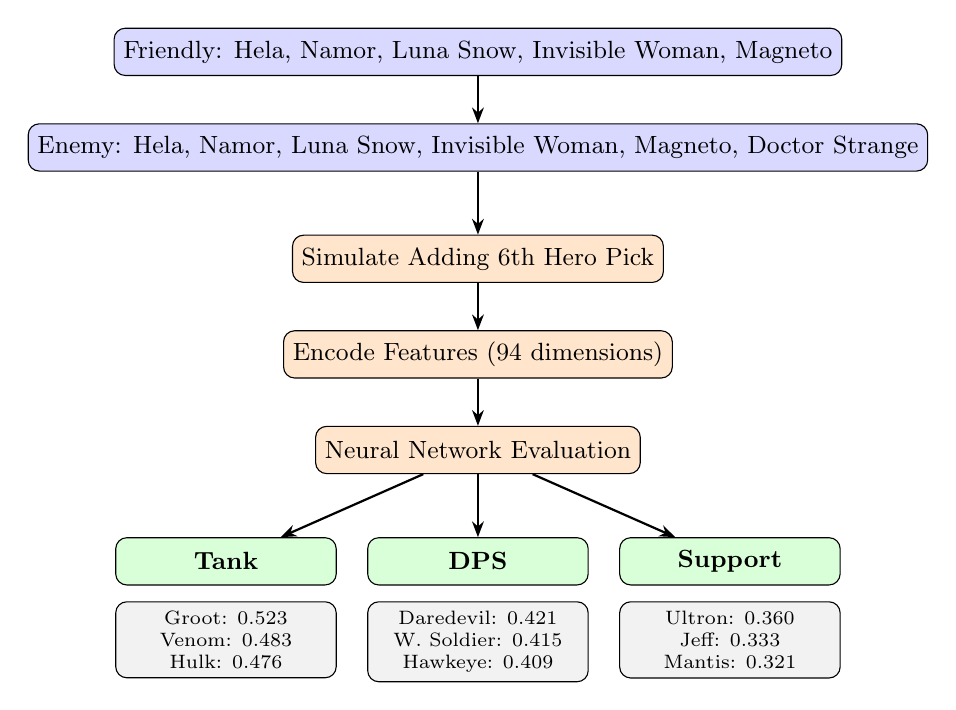
\begin{tikzpicture}[
        node distance=0.6cm,
        box/.style={rectangle, draw, rounded corners, minimum width=3.5cm, minimum height=0.6cm, align=center, font=\small},
        inputbox/.style={box, fill=blue!15},
        processbox/.style={box, fill=orange!20},
        outputbox/.style={box, fill=green!15, minimum width=2.8cm},
        herobox/.style={rectangle, draw, rounded corners, minimum width=2.8cm, align=center, font=\scriptsize, fill=gray!10},
        arrow/.style={-{Stealth[length=2mm]}, thick}
    ]

    % Input Section
    \node[inputbox] (friendly) {Friendly: Hela, Namor, Luna Snow, Invisible Woman, Magneto};
    \node[inputbox, below=of friendly] (enemy) {Enemy: Hela, Namor, Luna Snow, Invisible Woman, Magneto, Doctor Strange};

    % Processing Section
    \node[processbox, below=0.8cm of enemy] (simulate) {Simulate Adding 6th Hero Pick};
    \node[processbox, below=of simulate] (encode) {Encode Features (94 dimensions)};
    \node[processbox, below=of encode] (nn) {Neural Network Evaluation};

    % Output Section - Role headers
    \node[outputbox, below=0.8cm of nn, xshift=-3.2cm] (tank) {\textbf{Tank}};
    \node[outputbox, below=0.8cm of nn] (dps) {\textbf{DPS}};
    \node[outputbox, below=0.8cm of nn, xshift=3.2cm] (support) {\textbf{Support}};

    % Recommendation results
    \node[herobox, below=0.2cm of tank] (tankres) {Groot: 0.523\\Venom: 0.483\\Hulk: 0.476};
    \node[herobox, below=0.2cm of dps] (dpsres) {Daredevil: 0.421\\W. Soldier: 0.415\\Hawkeye: 0.409};
    \node[herobox, below=0.2cm of support] (suppres) {Ultron: 0.360\\Jeff: 0.333\\Mantis: 0.321};

    % Arrows
    \draw[arrow] (friendly) -- (enemy);
    \draw[arrow] (enemy) -- (simulate);
    \draw[arrow] (simulate) -- (encode);
    \draw[arrow] (encode) -- (nn);
    \draw[arrow] (nn) -- (tank);
    \draw[arrow] (nn) -- (dps);
    \draw[arrow] (nn) -- (support);

    \end{tikzpicture}%
    }
    \caption{Hero Recommendation System workflow. Given team compositions, the system simulates each candidate hero, encodes features, and returns top 3 recommendations per role with win probabilities.}
    \label{fig:hero_recommendation}
\end{figure}

\subsection{SVM}
A Support Vector Machine (SVM) is a supervised machine learning method for classification which finds the hyperplane that divides the data into target classes while maximizing the margin from the boundary plane to the nearest points. As many datasets are not linearly separable in their original feature space, it is common practice to use a kernel function which implicitly maps the data into a higher dimension space in which the boundary is a hyperplane. The Radial Basis Function (RBF) kernel is a popular choice, mapping the data into an infinite-dimensional space and frequently enabling linear separation of the data. We began with this approach, but as we gathered more data the time to fit the model began to grow impractical (over 1 hour with 100,000 samples, implying a full day of training to fit to the final dataset). Therefore, we used the RBFSampler kernel approximation implemented in scikit-learn, which approximates a RBF feature map using random Fourier features as described in \cite{randomkitchensinks}, and fit a linear SVM classifier to the transformed data. This achieved nearly identical results as the fully kernelized approach on smaller subsets of our data, but was much more computationally efficient, being able to fit to the final dataset of over 300k items in roughly 1 minute. The hyperparameters $\gamma$ and n\_components of the RBF sampler were tuned via cross-validation, with peak performance being found with $\gamma$ set to scale inversely to the number of features and the calculated variance in the original data, and $n\_components = 48$.

\subsection{Individual Player Models}
We also developed SVM models for predicting match outcomes and season-long player performance based on individual player's match statistics. The first of these was a linear SVM classifier like the one described above, but only operating on a single player's data rather than the entire team's. This approach reached an accuracy of 67\% in classifying matches as a win or loss, compared to the 89\% accuracy of the model given the full team's data. This result emphasizes the team-based nature of the game, showing that in as many as one in three games a player could find their team losing despite individually performing very well, or winning while undercontributing to the team. We also trained SVM-based regression models in an attempt to predict a player's season-long Win/Loss ratio, peak ELO rating, and average ELO rating, based only on their average match statistics. Despite trying various adjustments, none of these models ultimately performed significantly better than random--$R^2$ values for each ranged from $0.06-0.14$. We believe it may be possible to construct models that better reflect player skill and can predict these outcomes, but we also believe that this result could demonstrate the efficacy of the online matchmaking system: a player may win many matches at first, creating an impressive statistical record and a high W/L ratio, but as their ELO rises and they are paired with increasingly skilled opponents, the expected tendency is for their performance to stabilize and eventually converge to 50/50. It is notable that the model predicting season-long average ELO was the most effective of the three, indicating that there is still some difference in performance between a high-ranked player and a low-ranked player even when their Win/Loss ratios have converged to a similar level. 

\subsection{Random Forest}
Random Forest is an ensemble learning method that constructs multiple decision trees during training and outputs the mode of their predictions. Each tree is trained on a bootstrap sample of the data with a random subset of features at each split, reducing overfitting through decorrelation. The final prediction is:
\[
\hat{y} = \text{mode}\{h_1(\mathbf{x}), h_2(\mathbf{x}), \ldots, h_T(\mathbf{x})\}
\]
where $h_t(\mathbf{x})$ is the prediction of tree $t$ and $T=100$ is the number of trees.

\textbf{Configuration:} We used 100 estimators with default scikit-learn parameters. The model was trained on 105 features: 19 team statistics (kills, deaths, damage, healing, etc.) and 86 hero composition features (43 heroes $\times$ 2 teams encoded as binary presence indicators). Training used an 80/20 split with 5-fold stratified cross-validation.

\subsection{XGBoost}
XGBoost (Extreme Gradient Boosting) is a sequential boosting algorithm where each tree corrects errors from previous trees using second-order gradient optimization. It employs regularization (L1/L2) and column subsampling to prevent overfitting. The objective function minimized is:
\[
\mathcal{L} = \sum_{i=1}^{n} l(y_i, \hat{y}_i) + \sum_{t=1}^{T} \Omega(f_t), \quad \Omega(f) = \gamma T + \frac{1}{2}\lambda \|w\|^2
\]
where $l$ is the logistic loss, $\Omega$ is the regularization term, $\gamma$ penalizes tree complexity, and $\lambda$ is L2 regularization on leaf weights $w$.

\textbf{Configuration:} We used 100 boosting rounds with learning rate 0.1, max depth 6, and 80\% column subsampling per tree. The objective function was binary logistic regression with evaluation metric set to AUC-ROC.

\subsection{CatBoost}
CatBoost (Category Boosting) extends gradient boosting with ordered boosting to reduce prediction shift and native handling of categorical features. It uses symmetric trees and applies L2 regularization on leaf values for stability. Ordered boosting computes unbiased gradients using a random permutation $\sigma$ of training examples:
\[
g_i = \frac{\partial L(y_i, F^{(\sigma, i-1)}(x_i))}{\partial F}, \quad F^{(\sigma, i-1)} = \sum_{j: \sigma(j) < \sigma(i)} f_j
\]
where gradients for example $i$ are computed using only preceding examples in the permutation.

\textbf{Configuration:} We used 100 iterations with default learning rate, depth 6, and L2 leaf regularization of 3. CatBoost's ordered boosting reduces overfitting without extensive hyperparameter tuning.

\subsection{Retrieval-Augmented Generation (RAG)}
We implemented a RAG pipeline to enable natural language exploration of match data. The system converts match records into text documents, embeds them using \texttt{mxbai-embed-large}, and stores vectors in ChromaDB with HNSW indexing. Document retrieval uses L2 (Euclidean) distance:
\[
d(q, d) = \|\mathbf{e}_q - \mathbf{e}_d\|_2 = \sqrt{\sum_{i=1}^{n}(e_{q,i} - e_{d,i})^2}
\]
where $\mathbf{e}_q$ and $\mathbf{e}_d$ are the embedding vectors for query $q$ and document $d$.

\textbf{Architecture:}
\begin{itemize}
    \item \textbf{Document Processing:} Each match is converted to a structured text document containing team compositions, performance statistics, and outcomes.
    \item \textbf{Meta Statistics:} Aggregate statistics (averages, hero win rates, damage/kill totals) are pre-computed and prioritized in prompts for accurate aggregate queries.
    \item \textbf{Retrieval:} On query, the top 100 similar documents are retrieved via L2 distance.
    \item \textbf{Generation:} Retrieved context is combined with meta statistics and passed to \texttt{llama3.1} for response generation.
\end{itemize}

\textbf{Winner Prediction:} For winner prediction, the RAG pipeline uses semantic search to retrieve the top 100 similar matches from 5,000 indexed documents. The query is constructed from match statistics (hero compositions, kills, deaths), embedded, and matched against the ChromaDB index. The top 10 retrieved matches are included in the LLM prompt as context for prediction. Testing on 100 randomly sampled matches achieved 61\% accuracy, while preliminary tests on 1,000 samples showed improved accuracy of approximately 80\%.

% ============================================================================
\section{Evaluation}
% ============================================================================

\subsection{Evaluation Metrics}

The primary metric used to evaluate the neural network was \textbf{accuracy}, defined as the proportion of matches for which the predicted winner matched the true winner. Accuracy was chosen because the classification task is binary and balanced after applying randomized team flipping during data cleaning.

In addition to accuracy, qualitative evaluation was performed for the hero recommendation system by observing whether the predicted win probabilities aligned with known competitive patterns such as role balance, synergy, and meta compositions.

\subsection{Results}

The trained neural network achieved the following performance:
\begin{itemize}
    \item \textbf{Training Accuracy:} 0.915
    \item \textbf{Validation Accuracy:} 0.913
    \item \textbf{Test Accuracy:} 0.915
\end{itemize}

The close alignment between training, validation, and test accuracy indicates that the model generalizes well and does not overfit the dataset. Two factors were particularly important in achieving this stability: randomized team flipping, which removed positional bias, and the exclusion of final score information from the input features, which prevented target leakage.

For the hero recommendation system, qualitative testing showed that familiar meta compositions consistently resulted in higher predicted win probabilities, while role-imbalanced or anti-synergistic drafts produced lower probabilities. These observations matched intuitive expectations from competitive play and suggest that the neural network learned structural relationships such as role composition and synergy rather than relying solely on surface-level statistics. (KD)

\begin{table}[H]
    \centering
    \caption{Model Comparison (330,914 matches)}
    \label{tab:results}
    \begin{tabular}{lccc}
        \toprule
        Model & Accuracy & AUC-ROC & F1-Score \\
        \midrule
        Neural Network & \textbf{91.50\%} & -- & -- \\
        SVM & 86.00\% & -- & -- \\
        Random Forest & 89.76\% & 96.94\% & 89.59\% \\
        XGBoost & 89.97\% & 97.16\% & 89.81\% \\
        CatBoost & 89.88\% & 97.05\% & 89.72\% \\
        RAG (LLM) & 61\%-80\% & -- & -- \\
        \bottomrule
    \end{tabular}
\end{table}

\subsubsection{RAG Query Examples}
The RAG system successfully answers natural language queries about match statistics:
\begin{itemize}
    \item \textit{``What is the average match duration?''} $\rightarrow$ 673 seconds (11.2 minutes)
    \item \textit{``What is the average K/D ratio?''} $\rightarrow$ 2.57
    \item \textit{``What is the average damage dealt per match?''} $\rightarrow$ 173,503 total (86,751 per team)
\end{itemize}

\subsection{Discussion}

\textbf{Tree-Based Models:} All three ensemble methods achieved approximately 90\% accuracy with minimal performance differences. XGBoost achieved the highest metrics (89.97\% accuracy, 97.16\% AUC-ROC), while CatBoost trained fastest (1.76s). The high AUC-ROC scores ($>$97\%) indicate strong class separation capability. Feature importance analysis revealed that deaths, kills, and final hits were the most predictive features across all models.

\textbf{Cross-Validation:} We employed 5-fold stratified cross-validation to ensure robust evaluation. Stratification maintained class balance across folds, critical given the balanced win/loss distribution after randomized team flipping. The low standard deviations ($\pm$0.08--0.13\%) across folds indicate stable model performance regardless of data partitioning (see Appendix~\ref{sec:appendix} for detailed CV results).

\textbf{RAG System:} The RAG pipeline achieved 61\% accuracy on 100 samples and approximately 80\% on 1,000 samples using semantic search---lower than tree-based methods but demonstrating that accuracy improves with larger sample sizes. This gap highlights that while RAG excels at natural language exploration of match statistics, structured ML models remain superior for pure prediction tasks. The RAG system's value lies in enabling non-technical exploration of match patterns rather than prediction accuracy.

% Figures
\begin{figure}[H]
    \centering
    \includegraphics[width=0.48\textwidth]{figures/model_comparison.png}
    \caption{Performance comparison of tree-based models.}
    \label{fig:model_comparison}
\end{figure}

% ============================================================================
\section{Conclusion}
% ============================================================================

\subsection{Summary}
The neural network was our best-performing model, and future work would focus on tuning that model to achieve even higher performance. One area in which other algorithms outperformed it is in predicting outcomes based solely on the heroes chosen for each team, where CatBoost shined, so a Hero Recommender based on that model could be more effective. The models making predictions based on individual player stats underperformed, but this may be inherent to the dataset. 

\subsection{Future Work}
Several directions could extend this research:
\begin{itemize}
    \item \textbf{RAG Scaling:} Our RAG winner prediction showed improved accuracy with larger sample sizes (61\% on 100 samples vs.\ 80\% on 1,000 samples). With additional computational resources, testing on larger sample sizes (10,000+ matches) could further improve accuracy and better characterize the RAG pipeline's prediction ceiling.
    \item \textbf{Before Match Prediction:} Extending models to predict outcomes before a match using partial game state data.
    \item \textbf{Hero Recommendation Enhancement:} Incorporating temporal meta shifts and player-specific performance history.
\end{itemize}

% Manual references:
\begin{thebibliography}{9}

\bibitem{ref1}
C. J. A. Cordova, C. V. A. Villaceran and C. F. Peña, \textit{Predicting League of Legends Match Outcomes Through Machine Learning Models Using Past Match Player Performance,} 2024 IEEE International Conference on Computing (ICOCO), Kuala Lumpur, Malaysia, 2024, pp. 522-527, doi: 10.1109/ICOCO62848.2024.10928259.

\bibitem{xiao2021wpgbdt}
H. Xiao, Y. Liu, D. Du, and Z. Lu. (2021). \textit{WP-GBDT: An Approach for Winner Prediction using Gradient Boosting Decision Tree}. IEEE International Conference on Big Data, pp. 5765--5769. DOI: 10.1109/BigData52589.2021.9671688

\bibitem{akhmedov2021dota2}
K. Akhmedov and A. Phan. (2021). \textit{Machine Learning Models for DOTA 2 Outcomes Prediction}. arXiv preprint arXiv:2105.09953.

\bibitem{gourdeau2020hero}
D. Gourdeau and L. Archambault. (2020). \textit{Discriminative Neural Network for Hero Selection in Professional Heroes of the Storm and DOTA 2}. IEEE Transactions on Games, vol. 12, no. 4, pp. 427--436. DOI: 10.1109/TG.2020.2972463

\bibitem{randomkitchensinks}
Rahimi, Ali and Recht, Benjamin (2008) \textit{Weighted sums of random kitchen sinks: replacing minimization with randomization in learning}. Proceedings of the 22nd International Conference on Neural Information Processing Systems, pp. 1313-1320. DOI: 10.5555/2981780.2981944

\bibitem{ref6}
L. M. Costa, A. C. C. Souza and F. C. M. Souza, "An Approach for Team Composition in League of Legends using Genetic Algorithm," 2019 18th Brazilian Symposium on Computer Games and Digital Entertainment (SBGames), Rio de Janeiro, Brazil, 2019, pp. 52-61, doi: 10.1109/SBGames.2019.00018.

\bibitem{scraping1}
A. Abodayeh, R. Hejazi, W. Najjar, L. Shihadeh and R. Latif, \textit{Web Scraping for Data Analytics: A BeautifulSoup Implementation}, 2023 Sixth International Conference of Women in Data Science at Prince Sultan University (WiDS PSU), Riyadh, Saudi Arabia, 2023, pp. 65-69, doi: 10.1109/WiDS-PSU57071.2023.00025.

\bibitem{scraping2}
G. Sharma, \textit{Web Crawling and Scraping: A Survey}, 2024 International Conference on Healthcare Innovations, Software and Engineering Technologies (HISET), Karad, India, 2024, pp. 190-192, doi: 10.1109/HISET61796.2024.00063.

\bibitem{pandaskill}
M. D. Bois, F. Parmentier, R. Puget, M. Tanti and J. Peltier, \textit{PandaSkill - Player Performance and Skill Rating in Esports: Application to League of Legends}, in IEEE Transactions on Games, doi: 10.1109/TG.2025.3581070.

\end{thebibliography}
% ============================================================================
\newpage
\appendix
\section{Appendix}
\label{sec:appendix}
% ============================================================================

\subsection{Cross-Validation Results}

Table~\ref{tab:cv_results} presents the 5-fold stratified cross-validation results for tree-based models. The low standard deviations demonstrate consistent performance across different data partitions.

\begin{table}[H]
    \centering
    \caption{5-Fold Stratified Cross-Validation Results}
    \label{tab:cv_results}
    \begin{tabular}{lcc}
        \toprule
        Model & Mean CV Accuracy & Std Dev \\
        \midrule
        Random Forest & 89.83\% & $\pm$0.08\% \\
        XGBoost & 90.01\% & $\pm$0.13\% \\
        CatBoost & 90.05\% & $\pm$0.13\% \\
        \bottomrule
    \end{tabular}
\end{table}

\subsection{Additional Figures}

\begin{figure}[H]
    \centering
    \begin{minipage}{0.48\textwidth}
        \centering
        \includegraphics[width=\textwidth]{figures/combined_roc.png}
        \caption{ROC curves for tree-based models showing strong discrimination ability (AUC $>$ 0.97).}
        \label{fig:roc_curves}
    \end{minipage}
    \hfill
    \begin{minipage}{0.48\textwidth}
        \centering
        \includegraphics[width=\textwidth]{figures/xgb_feature_importance.png}
        \caption{XGBoost feature importance ranking.}
        \label{fig:feature_importance}
    \end{minipage}
\end{figure}

\begin{figure}[H]
    \centering
    \includegraphics[width=0.32\textwidth]{figures/rf_confusion_matrix.png}
    \hfill
    \includegraphics[width=0.32\textwidth]{figures/xgb_confusion_matrix.png}
    \hfill
    \includegraphics[width=0.32\textwidth]{figures/catboost_confusion_matrix.png}
    \caption{Confusion matrices for tree-based models. Left: Random Forest. Center: XGBoost. Right: CatBoost. All models show balanced performance across both classes.}
    \label{fig:confusion_matrices}
\end{figure}

\end{document}
